\chapter{CƠ SỞ LÝ THUYẾT}

Chương này trình bày các cơ sở lý thuyết cùng thông tin về các phần cứng liên quan, tạo tiền đề cho việc hiện thực và phát triển ứng dụng điều khiển cánh tay robot.

\section{Cánh tay robot Denso VS-6577}

Đầu tiên, cánh tay robot Denso VS-6577 chỉnh là đối tượng điều khiển chính trong đồ án hiện tại. Cánh tay robot \href{https://www.denso-wave.com/en/robot/product/five-six/vs.html}{Denso VS-6577} là một trong những model robot công nghiệp sáu trục nổi bật của hãng Denso - thương hiệu hàng đầu Nhật Bản trong lĩnh vực tự động hóa và robot công nghiệp. Được thiết kế với mục tiêu tối ưu hóa hiệu suất, độ chính xác và khả năng vận hành linh hoạt, VS-6577 đáp ứng tốt các yêu cầu khắt khe của sản xuất hiện đại trong nhiều ngành công nghiệp khác nhau.

Denso VS-6577 thuộc dòng robot sáu trục (6-axis articulated robot), mô phỏng chuyển động linh hoạt của cánh tay con người, cho phép thực hiện các thao tác phức tạp như lắp ráp, hàn, sơn, kiểm tra chất lượng, đóng gói và vận chuyển sản phẩm. Với sự kết hợp giữa thiết kế cơ khí tối ưu, hệ thống điều khiển thông minh và khả năng tích hợp dễ dàng vào các dây chuyền sản xuất tự động, VS-6577 đã và đang được ứng dụng rộng rãi tại nhiều nhà máy trên toàn cầu, đặc biệt trong các lĩnh vực điện tử, ô tô, thực phẩm, dược phẩm và logistics.

\begin{figure}[H]
    \centering
    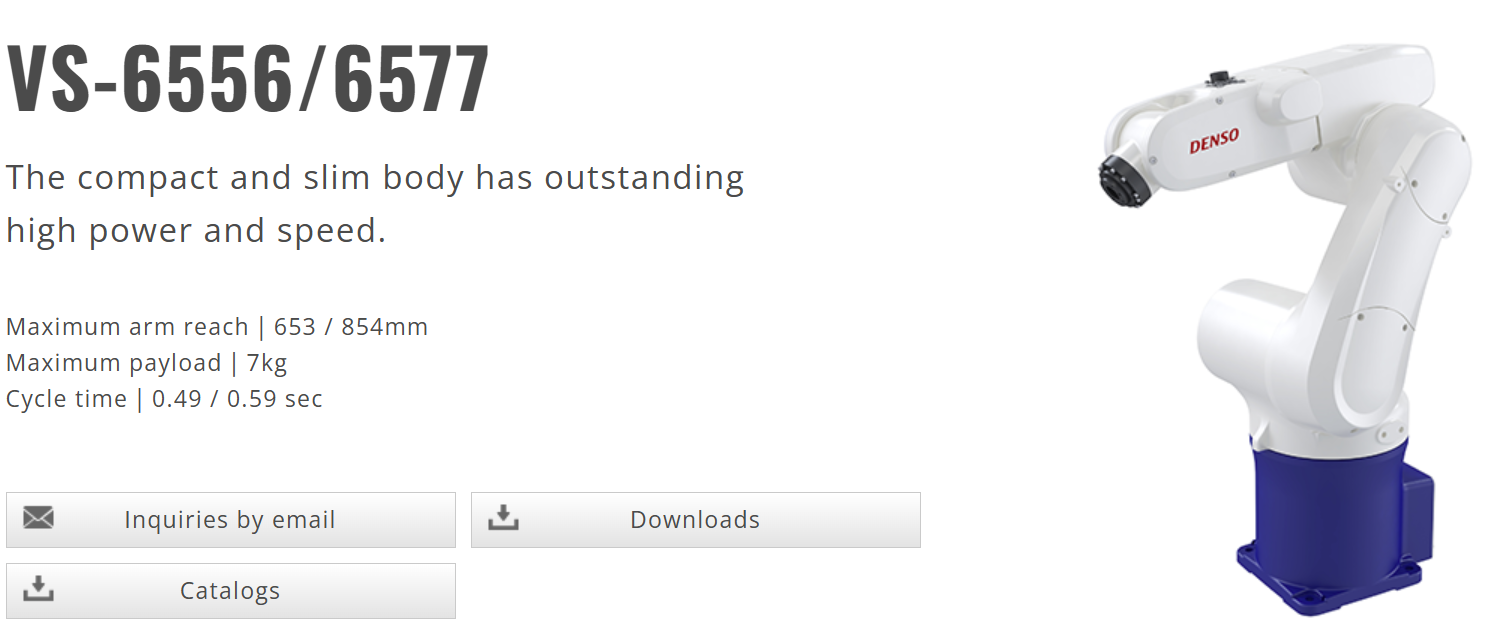
\includegraphics[width=1\linewidth]{Images/Methodologies/denso_arm_1.png}
    \caption{Cánh tay robot VS6577, hình ảnh lấy từ trang web nhà sản xuất}
    \label{fig:placeholder}
\end{figure}

Khi xem xét về đặc tả kĩ thuật của cánh tay, ta thấy thêm một số thông số ấn tượng về khả năng của cánh tay này:

\begin{longtblr}[
caption = {Thông số kĩ thuật của cánh tay Robot Denso VS-6577},
label = {tblr:my-table},
entry = {Thông số kĩ thuật của cánh tay Robot Denso VS-6577}
]{
hlines,vlines,
colspec = {X[1,c]X[3,l]},
columns = {valign = m},
}
Thông số kĩ thuật & Giá trị \\
Số trục & 6 \\
Độ dài cánh tay & 770mm \\
Độ lệch cánh tay & J1 (xoay): 75mm, J3 (cánh tay trước): 90mm \\
Vùng hoạt động tối đa & R = 934mm (tính phần mặt của end-effector), R=854mm (Tính phần trung tâm của J4, J5, J6) \\ 
Góc giới hạn & J1:±170°, \newline
                J2:+135°, -100°, \newline
                J3:+169°, -119°, \newline
                J4:±190°, \newline
                J5:±120°, \newline
                J6:±360° \\
Tải trọng tối đa & 7kg (với phần cổ cánh tay nghiêng xuống 1 góc khoảng 45°)\\
Nhận diện vị trí & Bộ Absolute Encoder\\
Động cơ xoay và phanh & AC motor cho toàn bộ các trục, phanh cho trục J2 tới J4\\
Khối lượng & ~ 36kg\\ 
Độ chính xác lặp lại & Với mỗi hướng X, Y và Z ±0.03mm\\
... & \\
\end{longtblr}

% 2 sub figure
\begin{figure}[H]
\centering
\begin{subfigure}{0.45\textwidth}
    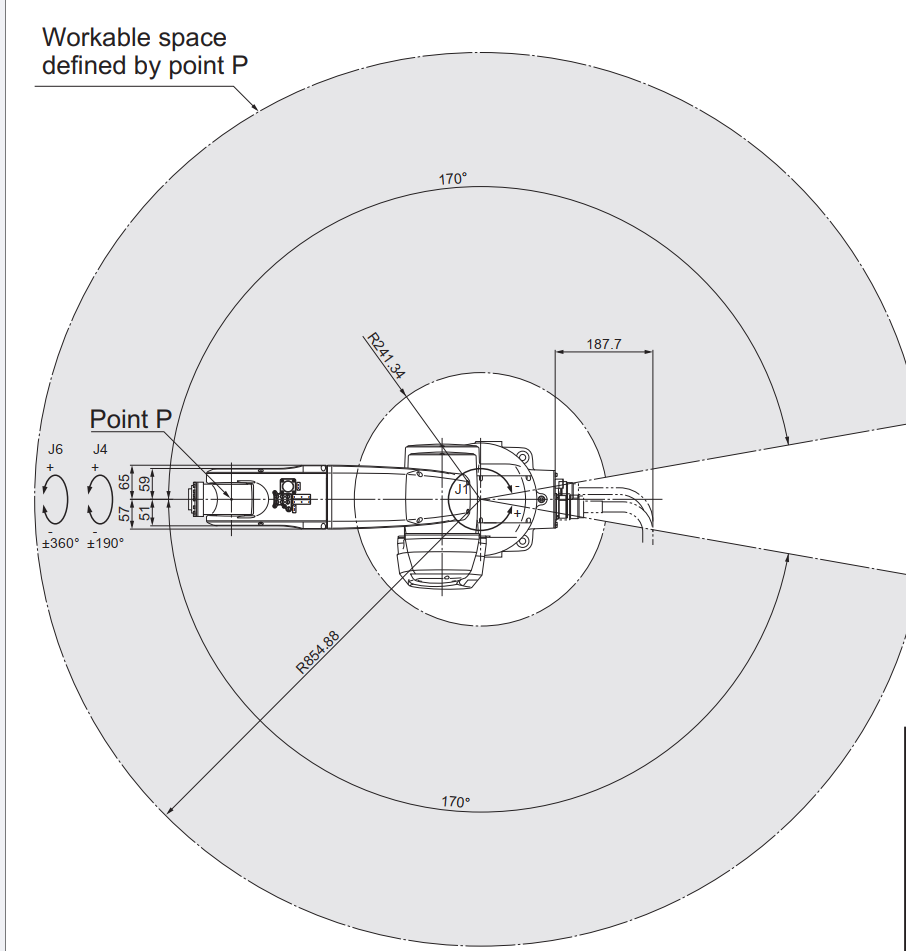
\includegraphics[width=\textwidth]{Images/Methodologies/denso_arm_2.png}
    %\caption{Train YOLO11-n}
\end{subfigure}
\hfill
\begin{subfigure}{0.45\textwidth}
    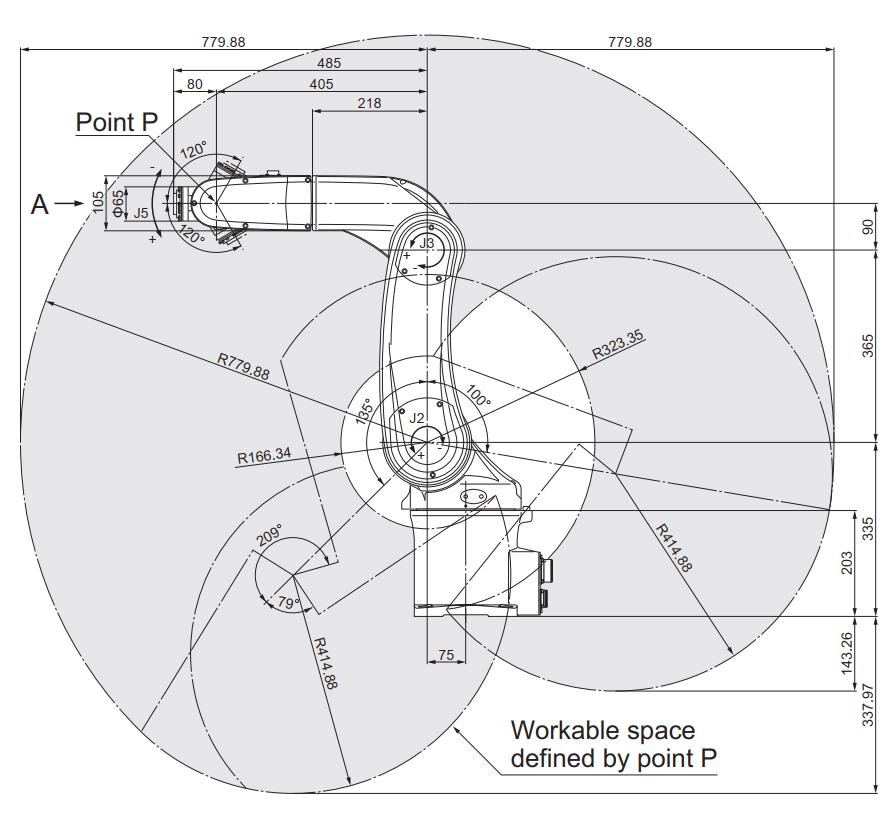
\includegraphics[width=\textwidth]{Images/Methodologies/denso_arm_3.png}
    %\caption{Train YOLO11-s}
\end{subfigure}
\hfill
\caption{Tầm hoạt động của cánh tay robot Denso từ nhà sản xuất}
\label{fig:denso_dimension}
\end{figure}

Với kích thước vừa phải và tương đối nhỏ gọn, cánh tay Denso VS6577 có sự linh hoạt tốt nhờ tầm hoạt động rộng ở từng trục, qua đó tạo nên vùng hoạt động lên tới 93.4cm tính cả phần mặt của end effector (phần đỉnh của cánh tay). Điều này giúp robot có thể dễ dàng tiếp cận và thao tác ở nhiều vị trí, góc độ khác nhau, đáp ứng tốt các yêu cầu ứng dụng đa dạng trong môi trường công nghiệp. Hơn nữa, độ chính xác lặp lại đạt ±0,03 mm (theo tài liệu kỹ thuật mới nhất), đảm bảo các thao tác lặp đi lặp lại đều đạt độ chính xác gần như tuyệt đối. Cánh tay Denso VS6577 là một lựa chọn tuyệt vời cho các ứng dụng trong môi trường nhà máy, công nghiệp, nơi sự chính xác và ổn định là yếu tố then chốt.

\section{Máy tính điều khiển RC5}

Bộ điều khiển RC5 của DENSO là một trong những giải pháp điều khiển robot công nghiệp nổi bật, được sử dụng rộng rãi trong các dây chuyền tự động hóa hiện đại trên toàn cầu. Được phát triển bởi DENSO – tập đoàn hàng đầu Nhật Bản về công nghệ tự động hóa và robot công nghiệp – RC5 không chỉ đáp ứng các tiêu chuẩn kỹ thuật khắt khe mà còn mang lại sự linh hoạt, độ tin cậy và khả năng tích hợp cao cho nhiều ứng dụng sản xuất khác nhau.

Hiện tại, bộ điều khiển Denso RC5 đang đóng vai trò điều khiển trực tiếp các trục xoay của cánh tay robot VS-6577. 

\begin{figure}[H]
    \centering
    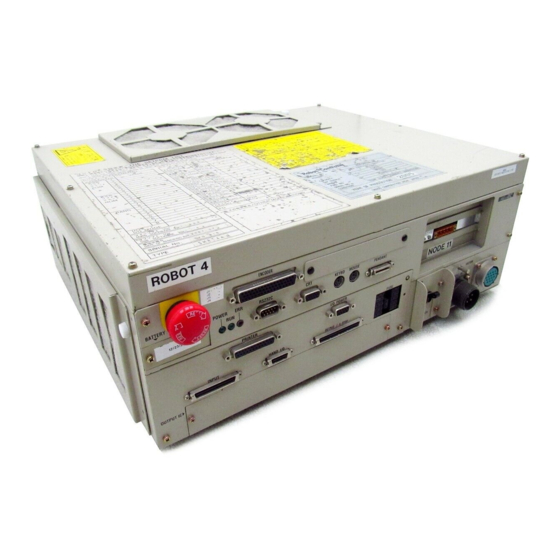
\includegraphics[width=0.7\linewidth]{Images/Methodologies/rc5_image.jpg}
    \caption{Máy tính điều khiển RC5}
    \label{fig:placeholder}
\end{figure}

Bộ điều khiển RC5 được thiết kế với nhiều phiên bản khác nhau, nhằm mục tiêu tối ưu cho từng loại robot khác nhau. Trong trường hợp hiện tại, bộ điều khiển RC5 có mã là RC5-VSE6B, trong đó "VSE" tức tương thích với dòng robot VS-E, "6" cho biết số trục điều khiển được là 6 trục, và "B" cho biết encoder được kết nối tới cổng CN12. Chi tiết vị trí của các cổng đầu vào sẽ được trình bày ở ảnh dưới:

\begin{figure}[H]
    \centering
    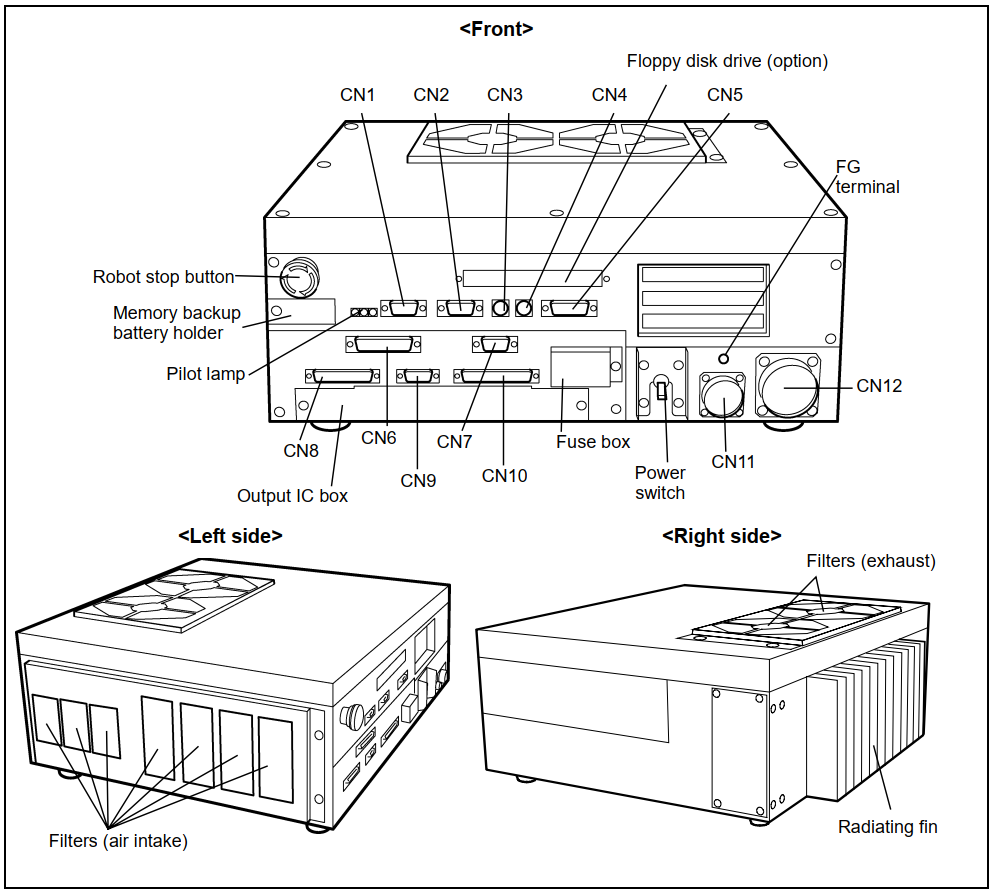
\includegraphics[width=1\linewidth]{Images/Methodologies/rc5_design.png}
    \caption{Vị trí các cổng nối của máy RC5}
    \label{fig:placeholder}
\end{figure}

\begin{longtblr}[
caption = {Ý nghĩa các cổng đầu vào trên máy điều khiển RC5},
label = {tblr:my-table},
entry = {Ý nghĩa các cổng đầu vào trên máy điều khiển RC5}
]{
hlines,vlines,
colspec = {X[1,c]X[1.5,c]X[2,l]X[1,c]X[1,c]X[2,l]},
columns = {valign = m},
}
\textbf{Số hiệu} & \textbf{Ký hiệu} & \textbf{Tên} & \textbf{Số hiệu} & \textbf{Ký hiệu} & \textbf{Tên} \\
CN1 & RS232C & Cổng giao tiếp nối tiếp & CN7 & I/O POWER & Cổng nguồn cho I/O \\
CN2 & CRT & Cổng màn hình CRT & CN8 & INPUT & Cổng đầu vào người dùng hoặc hệ thống (PLC) \\
CN3 & KEYBD & Cổng bàn phím & CN9 & HAND I/O & Cổng I/O cho End effector \\
CN4 & MOUSE & Cổng chuột PS/2 & CN10 & OUTPUT & Cổng đầu ra người dùng hoặc hệ thống (PLC) \\
CN5 & PENDANT & Cổng tay dạy (teach pendant) & CN11 & INPUT AC & Cổng nguồn xoay chiều \\
CN6 & PRINTER & Cổng máy in (không sử dụng) & CN12 & MOTOR & Cổng động cơ/bộ mã hóa \\
\end{longtblr}

Với việc có một lượng lớn các cổng kết nối, người dùng có sự linh hoạt trong việc tích hợp nó vào chu trình điều khiển hiện có. Không chỉ đơn thuần là điều khiển cánh tay robot, RC5 cũng có thể được sử dụng để điều khiển thêm các đầu gắp (end effector), kết nối với hệ thống PLC, kết nối với thiết bị "teach pendant", điều khiển I/O của nhiều thiết bị khác và hơn hết là cho phép kết nối với PC / thiết bị hỗ trợ quan sát (vision device) thông qua cổng giao tiếp RS232. 

\begin{longtblr}[
caption = {Bảng thông số kĩ thuật của máy điều khiển RC5 cho cánh tay robot VS-6577},
label = {tblr:my-table},
entry = {Bảng thông số kĩ thuật của máy điều khiển RC5 cho cánh tay robot VS-6577}
]{
hlines,vlines,
colspec = {X[1,c]X[3,l]},
columns = {valign = m},
}
\textbf{Mục} & \textbf{Thông số kỹ thuật} \\
Hệ thống điều khiển (GHI CHÚ 1) & PTP, CP tuyến tính 3 chiều, tròn 3 chiều \\
Số trục điều khiển (GHI CHÚ 1) & V*-D/E: Tối đa 6 trục đồng thời \\
Hệ thống truyền động & Tất cả các trục: Servo AC kỹ thuật số hoàn toàn \\
Dung lượng bộ nhớ & 1.25 MB (tương đương 5000 bước, 13.000 điểm) \\
Ngôn ngữ sử dụng & Ngôn ngữ robot DENSO (tuân theo SLIM) \\
Số chương trình dạy có thể tải vào bộ nhớ & 255 \\
Hệ thống dạy học & 1) Dạy từ xa 2) Nhập số liệu (MDI) \\
\SetCell[r=2]{c} Tín hiệu ngoài (I/O) & Tín hiệu vào: 20 điểm mở cho người dùng (PLC 12, tay vào 8) + 36 điểm hệ thống cố định\\ 
 & Tín hiệu ra: 32 điểm mở cho người dùng (PLC 24, tay ra 8) + 33 điểm hệ thống cố định \\
\SetCell[r=2]{c} Giao tiếp ngoài & RS-232C: 1 đường \\ 
& Ethernet: 1 đường (tùy chọn) \\
Chức năng hẹn giờ & 0.02 đến 10 giây (đơn vị 1/60 giây) \\
Chức năng tự chẩn đoán & Quá giới hạn, lỗi servo, lỗi bộ nhớ, lỗi đầu vào, v.v. \\
\SetCell[r=2]{c} Hiển thị lỗi & Mã lỗi hiển thị qua I/O ngoài hoặc bảng điều khiển (tùy chọn) \\
 & Thông báo lỗi hiển thị bằng tiếng Anh trên tay dạy (tùy chọn) \\
Nguồn điện & RC5 cho VS-D/E, H*-D/E, XYC-D: 1 pha, 230 VAC-10\% đến 230 VAC+10\%, 50/60 Hz\\
Công suất tiêu thụ (GHI CHÚ 1) & VS-E: 1.9 kVA\\ 
\SetCell[r=2]{c} Điều kiện môi trường (khi hoạt động) & Nhiệt độ: 0 đến 40°C\\ 
 & Độ ẩm: Dưới 90\% RH (không ngưng tụ) \\
Mức độ bảo vệ & IP20 \\
\SetCell[r=3]{c} Cáp (tùy chọn) & Cáp điều khiển robot: VS-D, H*-D, XYC-D: 3 m, 6 m (tùy chọn) \\ 
& Cáp I/O: 8 m, 15 m\\ 
& Cáp nguồn: 5 m \\
Khối lượng & VS-D/E, VC-E, HS-E: Khoảng 17 kg\\
\end{longtblr}

\begin{itemize}
    \item \textbf{Hệ thống điều khiển} của RC5 hỗ trợ các chế độ chuyển động PTP (Point-to-Point), CP (Continuous Path) với khả năng điều khiển tuyến tính và tròn trong không gian 3 chiều. Điều này cho phép RC5 đáp ứng tốt các yêu cầu chuyển động phức tạp trong các ứng dụng lắp ráp, hàn, sơn, hoặc xử lý vật liệu chính xác cao.
    \item \textbf{Dung lượng bộ nhớ} 1.25 MB cho phép lưu trữ tới 5000 bước chương trình và 13.000 điểm tọa độ, đáp ứng nhu cầu lập trình các chu trình phức tạp, đa nhiệm vụ. Số lượng chương trình dạy tối đa là 255, giúp người dùng dễ dàng quản lý và chuyển đổi giữa các tác vụ sản xuất khác nhau.
    \item \textbf{Khả năng tự chuẩn đoán lỗi} cũng là một tính năng quan trọng để đảm bảo việc vận hành robot được an toàn.
    \item Về \textbf{Ngôn ngữ sử dụng}, Ngôn ngữ robot DENSO, hay còn gọi là WINCAPS phiên bản 1 được sử dụng để có thể lập trình ngay trên máy RC5, tận dụng những hàm hỗ trợ về nhiều khía cạnh như input/ouput, ghi log, chuyển động cánh tay robot gồm thay đổi góc xoay, thay đổi tốc độ, thay đổi gia tốc, thay đổi vị trí.... Ngôn ngữ lập trình này cũng cung cấp đầy đủ các công cụ lập trình cần thiết như vòng lặp, điều kiện, khai báo và sử dụng biến, biến toàn cục và biến cục bộ. 
\end{itemize}
  
Tóm lại, máy tính điều khiển RC5 là một bộ điều khiển không thể thiếu để hoạt động cùng với cánh tay robot VS-6577, giúp giải quyết sự phức tạp trong điều khiển các bộ motor trong cánh tay robot sao cho mượt mà, hiệu quả và chính xác, đáp ứng những yêu cầu khắc khe về thời gian cũng như độ tin cậy trong phần lớn những ứng dụng trong môi trường công nghiệp.

\section{Gripper-A và Driver-Hat-A}

\subsection{Tay gắp Gripper-A}

Tay gắp (gripper) là một loại thiết bị cuối (end-effector) phổ biến được lắp vào đầu cánh tay robot, có vai trò trực tiếp tương tác với đối tượng trong môi trường làm việc. Tùy theo ứng dụng, gripper có thể có nhiều dạng khác nhau: kiểu ngón tay song song (parallel jaw gripper), kiểu hút chân không, kiểu nam châm điện, hay thiết kế lấy cảm hứng từ bàn tay người. Trong đề tài này, tay gắp được chọn là loại \textbf{parallel jaw gripper} (hai hàm song song) với cơ cấu điều khiển bằng servo motor.

\begin{figure}[H]
    \centering
    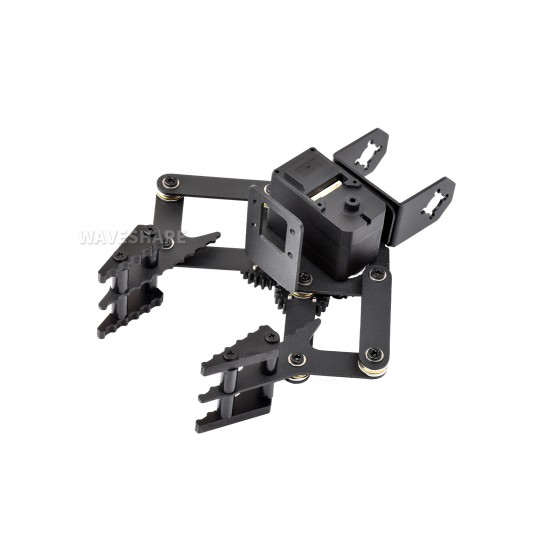
\includegraphics[width=0.6\linewidth]{Images/Methodologies/gripper_a.jpg}
    \caption{Tay gắp Gripper-A}
    \label{fig:gripper_a}
\end{figure}

Tay gắp được điều khiển thông qua một servo motor duy nhất, có tên khớp (joint) là \lstinline[style=inlinecode]{gripper_gear_right_joint}. Phạm vi chuyển động của servo nằm trong khoảng từ \textbf{5°} (vị trí đóng hoàn toàn, tương đương 0.087266 rad) đến \textbf{85°} (vị trí mở hoàn toàn, tương đương 1.48353 rad). Cơ cấu bánh răng bên trong tay gắp chuyển đổi góc xoay của servo thành chuyển động tịnh tiến của hai hàm gắp theo hướng đối xứng nhau, đảm bảo vật thể được kẹp giữ ở chính giữa.

\subsection{Driver-Hat-A}

Driver-Hat-A là một bo mạch điều khiển servo được thiết kế dưới dạng \textit{hat} (mũ gắn lên), tương thích với các máy tính nhúng như Raspberry Pi hoặc Jetson. Bo mạch này đóng vai trò cầu nối trung gian giữa PC Controller và servo motor bên trong tay gắp, nhận lệnh điều khiển qua giao tiếp \textbf{UART} (cổng \lstinline[style=inlinecode]{/dev/ttyACM0}, tốc độ 115200 bps) và xuất tín hiệu điều khiển servo tương ứng.

\begin{figure}[H]
    \centering
    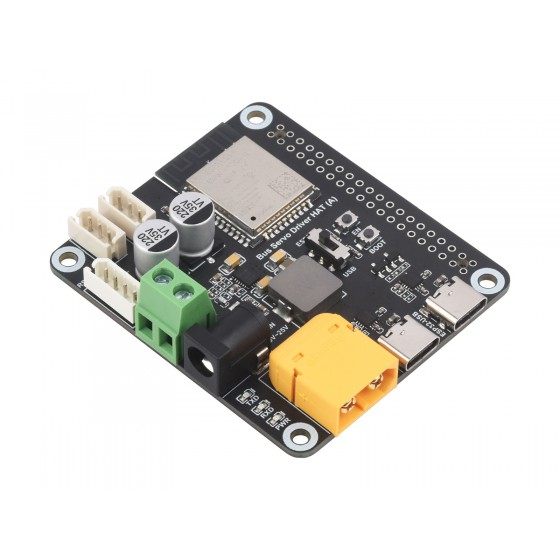
\includegraphics[width=0.5\linewidth]{Images/Methodologies/driver_hat_a.jpg}
    \caption{Bo mạch Driver-Hat-A}
    \label{fig:driver_hat_a}
\end{figure}

\textbf{Giao thức truyền thông JSON}

Driver-Hat-A sử dụng giao thức lệnh dạng chuỗi \textbf{JSON} (JavaScript Object Notation), giúp lệnh truyền đi dễ đọc, dễ kiểm tra và mở rộng. Lệnh điều khiển vị trí servo có định dạng:

\begin{lstlisting}[language=json]
{"T":121,"angle":0.67,"spd":100,"acc":10}
\end{lstlisting}

Trong đó:
\begin{itemize}
    \item \lstinline[style=inlinecode]{"T":121}: Mã lệnh điều khiển vị trí servo.
    \item \lstinline[style=inlinecode]{"angle"}: Góc xoay mục tiêu của servo tính bằng \textbf{radian}.
    \item \lstinline[style=inlinecode]{"spd"}: Tốc độ xoay, trong khoảng từ 0 đến 4096 (0 = tốc độ tối đa).
    \item \lstinline[style=inlinecode]{"acc"}: Gia tốc, trong khoảng từ 0 đến 254 (0 = gia tốc tối đa).
\end{itemize}

Để truy vấn trạng thái hiện tại của servo, PC Controller gửi lệnh:
\begin{lstlisting}[language=json]
{"T":105}
\end{lstlisting}

Driver-Hat-A sẽ phản hồi với gói tin chứa đầy đủ thông tin:
\begin{lstlisting}[language=json]
{"T":1051,"pos":3138,"speed":0,"load":-104,"voltage":124,
 "current":4,"temper":45,"mode":0}
\end{lstlisting}

Trường \lstinline[style=inlinecode]{"pos"} chứa vị trí hiện tại của servo dưới dạng \textbf{giá trị encoder step} (không phải góc độ trực tiếp). Để chuyển đổi sang góc độ (đơn vị độ), ta áp dụng công thức:

\begin{align*}
angle\_deg = (pos - 1024) \times \frac{360}{4096}
\end{align*}

Ngoài vị trí, các thông số phụ như \lstinline[style=inlinecode]{speed} (vận tốc), \lstinline[style=inlinecode]{load} (tải trọng), \lstinline[style=inlinecode]{voltage} (điện áp), \lstinline[style=inlinecode]{current} (dòng điện) và \lstinline[style=inlinecode]{temper} (nhiệt độ) cũng được trả về, giúp hệ thống có thể phát hiện sự cố trong quá trình hoạt động. Đặc biệt, giá trị \lstinline[style=inlinecode]{load} rất hữu ích để phát hiện khi tay gắp đang kẹp vật thể (tải trọng tăng đột biến), hỗ trợ cơ chế dừng tự động tránh làm hỏng vật gắp.


\section{Khái niệm về động học robot}

Động học (kinematics) là một nhánh của cơ học nghiên cứu về chuyển động của vật thể mà không xét đến nguyên nhân gây ra chuyển động đó (tức là không xét đến lực). Trong robot học, động học tập trung vào việc mô tả vị trí, hướng, vận tốc và gia tốc của các bộ phận robot dựa trên các biến khớp (joint variables) và cấu trúc hình học của hệ thống.

Đối với cánh tay robot sáu trục như Denso VS-6577, toàn bộ cấu trúc cơ khí có thể được mô hình hóa như một chuỗi các khâu cứng nối tiếp nhau qua các khớp xoay (revolute joints). Trạng thái của robot tại mọi thời điểm được đặc trưng bởi vector các giá trị khớp $\mathbf{q} = [q_1, q_2, q_3, q_4, q_5, q_6]^T$, trong đó $q_i$ là góc xoay của khớp thứ $i$. Có hai bài toán cơ bản trong động học robot: \textbf{động học thuận} và \textbf{động học nghịch}.

\subsection{Động học thuận}

Động học thuận (Forward Kinematics - FK) là quá trình xác định vị trí và hướng của end-effector trong không gian Cartesian dựa trên tập giá trị khớp đã biết và các tham số hình học của robot. Đây là bài toán có \textbf{nghiệm duy nhất}: với một cấu hình khớp xác định, chỉ tồn tại đúng một tư thế tương ứng của end-effector.

Phương pháp phổ biến nhất để giải bài toán động học thuận là sử dụng \textbf{quy ước Denavit–Hartenberg (DH)}. Theo quy ước này, mỗi khớp $i$ được gán một hệ tọa độ cục bộ, và mối quan hệ giữa hai hệ tọa độ liền kề được mô tả bởi bốn tham số DH: $a_i$, $\alpha_i$, $d_i$, $\theta_i$. Ma trận biến đổi đồng nhất giữa hai khâu liền kề được xác định bởi:

\begin{equation}
^{i-1}T_i = 
\begin{bmatrix}
\cos\theta_i & -\sin\theta_i\cos\alpha_i &  \sin\theta_i\sin\alpha_i & a_i\cos\theta_i \\
\sin\theta_i &  \cos\theta_i\cos\alpha_i & -\cos\theta_i\sin\alpha_i & a_i\sin\theta_i \\
0            &  \sin\alpha_i             &  \cos\alpha_i             & d_i             \\
0            &  0                        &  0                        & 1
\end{bmatrix}
\end{equation}

Tư thế của end-effector so với hệ tọa độ gốc được tính bằng tích liên tiếp của các ma trận biến đổi:

\begin{equation}
^0T_6 = {^0T_1} \cdot {^1T_2} \cdot {^2T_3} \cdot {^3T_4} \cdot {^4T_5} \cdot {^5T_6}
\end{equation}

Ma trận $^0T_6 \in \mathbb{R}^{4 \times 4}$ là \textbf{ma trận biến đổi đồng nhất} chứa đầy đủ thông tin về vị trí (cột cuối, 3 hàng đầu) và hướng (ma trận con $3\times3$ góc trên trái) của end-effector. Động học thuận là nền tảng cho việc hiển thị, mô phỏng robot và cũng là cơ sở để kiểm tra kết quả của bài toán động học nghịch.

\subsection{Động học nghịch}

Động học nghịch (Inverse Kinematics - IK) là quá trình xác định tập giá trị khớp $\mathbf{q}$ cần thiết để đưa end-effector đến một tư thế mong muốn $\mathbf{x} = [x, y, z, \phi, \psi, \theta]^T$ cho trước trong không gian Cartesian. Đây là bài toán \textbf{ngược với} động học thuận, thường phức tạp hơn nhiều vì:

\begin{itemize}
    \item Bài toán có thể có \textbf{nhiều nghiệm} (nhiều cấu hình khớp khác nhau đều đưa end-effector đến cùng một tư thế), \textbf{một nghiệm duy nhất}, hoặc \textbf{không có nghiệm} (tư thế mục tiêu nằm ngoài vùng làm việc).
    \item Đối với robot 6 bậc tự do thông thường, có thể tồn tại đến 16 nghiệm IK khác nhau tùy theo cấu hình cơ học.
    \item Hệ phương trình phi tuyến không phải lúc nào cũng có nghiệm giải tích (closed-form) và thường phải dùng phương pháp số (iterative).
\end{itemize}

Có hai nhóm phương pháp chính để giải bài toán IK:

\begin{enumerate}
    \item \textbf{Phương pháp giải tích (Closed-form / Analytical IK)}: Khai thác cấu trúc hình học đặc thù của robot (ví dụ: ba trục cuối giao nhau tại một điểm – cấu hình cổ tay cầu - spherical wrist) để tìm nghiệm dạng công thức toán học. Phương pháp này cho kết quả nhanh và chính xác nhưng chỉ áp dụng được cho một số kiểu robot nhất định.
    
    \item \textbf{Phương pháp số (Numerical IK)}: Sử dụng các thuật toán lặp như phương pháp Jacobian pseudo-inverse, thuật toán gradient descent hoặc các phương pháp tối ưu hóa để hội tụ đến nghiệm. Phương pháp này tổng quát hơn nhưng có thể chậm hơn, phụ thuộc vào điểm khởi tạo và có thể không hội tụ gần các điểm kỳ dị (singularity).
\end{enumerate}

Trong đề tài, bài toán IK được giải quyết thông qua thư viện plugin của MoveIt2, cụ thể là \textbf{KDL Kinematics Plugin} (\lstinline[style=inlinecode]{kdl_kinematics_plugin/KDLKinematicsPlugin}) – một solver IK số dựa trên thư viện Kinematics and Dynamics Library của Orocos, với thời gian tìm kiếm và timeout được cấu hình trong file \lstinline[style=inlinecode]{kinematics.yaml}:

\begin{lstlisting}
denso_arm:
  kinematics_solver: kdl_kinematics_plugin/KDLKinematicsPlugin
  kinematics_solver_search_resolution: 0.005
  kinematics_solver_timeout: 0.005
\end{lstlisting}

Khi ứng dụng VR hoặc module Remote Control yêu cầu cánh tay di chuyển đến một tư thế Cartesian xác định, MoveIt2 sẽ tự động gọi plugin IK này để tính toán cấu hình khớp tương ứng, sau đó lập kế hoạch quỹ đạo an toàn và thực thi.


\section{Giao thức UART}

UART (Universal Asynchronous Receiver/Transmitter – Bộ truyền nhận dữ liệu nối tiếp bất đồng bộ) là một trong những giao thức truyền thông nối tiếp cơ bản và lâu đời nhất, được sử dụng rộng rãi trong lĩnh vực điện tử, hệ thống nhúng, máy tính và các thiết bị ngoại vi. Ra đời từ những năm 1970 với sự xuất hiện của chip WD1402A của Western Digital, UART đã trở thành nền tảng cho việc truyền dữ liệu giữa các thiết bị số mà không cần đến tín hiệu đồng hồ chung.

Về bản chất, UART là một phần cứng hoặc module tích hợp trong vi điều khiển, máy tính, hoặc có thể là một IC độc lập, đảm nhiệm việc chuyển đổi dữ liệu song song từ CPU hoặc bus dữ liệu thành dữ liệu nối tiếp để truyền đi, và ngược lại, chuyển đổi dữ liệu nối tiếp nhận được thành song song để xử lý tiếp theo. Giao tiếp UART sử dụng hai dây chính: TX (Transmit – truyền) và RX (Receive – nhận), cùng với dây nối đất chung, giúp đơn giản hóa kết nối vật lý giữa các thiết bị.

\begin{figure}[H]
    \centering
    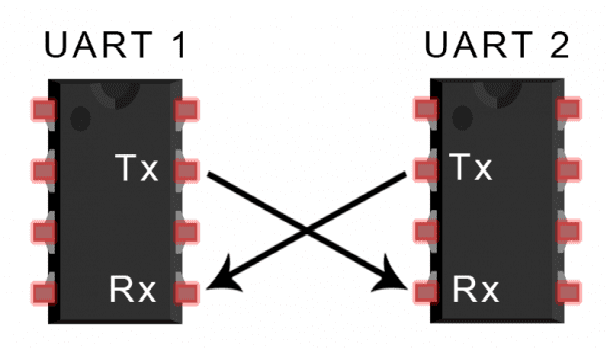
\includegraphics[width=0.8\linewidth]{Images/Methodologies/uart_2.png}
    \caption{Kết nối UART}
    \label{fig:placeholder}
\end{figure}

Điểm nổi bật của UART là khả năng truyền dữ liệu không đồng bộ, tức là không cần tín hiệu clock chung giữa hai thiết bị truyền và nhận. Thay vào đó, các thiết bị phải được cấu hình cùng tốc độ truyền (baud rate) và cùng định dạng khung dữ liệu để đảm bảo việc truyền nhận chính xác. Để nhận biết việc nhận dữ liệu, UART sử dụng các start bit và stop bit vào gói dữ liệu, giúp xác định điểm bắt đầu và điểm kết thúc của một dữ liệu được truyền trên dường dây.

Định dạng của một gói tin UART thường sẽ gồm 4 phần: Start bit, data frame, parity và stop bit:

\begin{figure}[H]
    \centering
    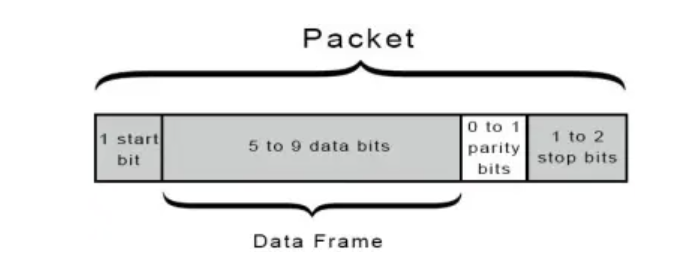
\includegraphics[width=0.8\linewidth]{Images/Methodologies/uart_1.png}
    \caption{Định dạng một gói tin (package) của UART}
    \label{fig:placeholder}
\end{figure}

\begin{enumerate}
    \item \textbf{Start bit}: Thông thường, đường truyền dữ liệu UART sẽ ở mức điện áp cao khi không có dữ liệu. Lúc bắt đầu truyền dữ liệu, UART sẽ kéo đường truyền xuống mức thấp trong một chu kì xung nhịp. Đây chính là Start bit của quá trình truyền nhận. Thiết bị UART ở phía nhận khi nhận thấy tín hiệu xuống thấp lần đầu tiên sẽ bắt đầu đọc các dữ liệu được truyền sau đó
    \item \textbf{Data Frame}: Đây là khu vực chứa dữ liệu cần truyền. Độ dài của dữ liệu có thể từ 5 tới 9 bit, với 9 bit trong trường hợp không sử dụng Parity bit. 
    \item \textbf{Parity Bit}: Parity bit chỉ có một bit, cho biết số lượng bit 1 trong khung dữ liệu là số chẵn hay số lẻ. Mục tiêu của Parity bit là bảo đảm sự toàn vẹn dữ liệu ở mức tương đối, như một cách để thiết bị nhận biết rằng có bất kì dữ liệu nào đã bị thay đổi trong quá trình truyền hay không. 
    \item \textbf{Stop bits}: Stop bits có độ dài từ 1 tới 2 bit, khi đó UART sẽ gửi tín hiệu điện áp từ thấp lên cao trong ít nhất hai bit, đánh dấu sự kết thúc của gói tin truyền nhận.
\end{enumerate}

\textbf{Ưu điểm của giao thức UART}

Khi nhắc tới UART, ta có thể nhận thấy ngay nhiều ưu điểm của giao thức này như:

\begin{itemize}
    \item Kết nối đơn giản, chỉ sử dụng hai dây truyền dữ liệu cho giao tiếp điểm - điểm (Point to Point)
    \item Không cần đồng bộ với xung clock để hoạt động
    \item Có cơ chế kiểm tra lỗi thông qua bit chẵn lẻ
    \item Tốc độ truyền đa dạng, với baud rate từ 110 bps lên tới 921600 bps
    \item Phương pháp truyền đơn giản và giá thành thấp
\end{itemize}

\textbf{Nhược điểm của giao thức UART}

Tuy vậy, sự đơn giản của UART cũng mang cho nó một số nhược điểm so với các giao thức khác:

\begin{itemize}
    \item Kích thước dữ liệu trong mỗi gói tin nhỏ, chỉ tối đa 9 bit
    \item Chỉ phù hợp cho kết nối Point to Point. Không phù hợp trong kết nối dạng Master-Slave cần điều khiển nhiều thiết bị cùng lúc
    \item Tốc độ tối đa sẽ thấp hơn SPI, I2C, bị ảnh hưởng bởi chiều dài dây và khả năng bị nhiễu
    \item Yêu cầu hai thiết bị phải có cùng baud rate, hoặc ít nhất sự chênh lệnh không vượt quá 10\%
\end{itemize}

\section{ROS2 - Robot Operating System}

ROS2 (Robot Operating System) là một hệ thống phần mềm mã nguồn mở dành cho robot, được phát triển bởi Willow Garage và hiện đang được duy trì bởi Open Robotics. Dù gọi mình là một hệ điều hành (Operating System), ROS 2 không thực sự là một hệ điều hành, mà cung cấp một khung làm việc (framework) gồm vô số các công cụ mạnh mẽ để phát triển các ứng dụng robot, cung cấp các công cụ và thư viện để giúp lập trình viên tạo ra các ứng dụng điều khiển robot, phân tích dữ liệu, xử lý hình ảnh và video, và tương tác với các thiết bị ngoại vi.

ROS 2 được thiết kế để hoạt động trên nhiều hệ điều hành khác nhau, bao gồm Linux, macOS và Windows. Nó cũng được tích hợp sẵn với các thư viện và công cụ phổ biến như OpenCV, PCL (Point Cloud Library) và TensorFlow.

ROS 2 có nhiều ưu điểm, bao gồm:
\begin{itemize}
    \item Tích hợp dễ dàng: ROS 2 có thể kết nối với các thiết bị phần cứng và phần mềm khác một cách dễ dàng, giúp người dùng tập trung vào phát triển ứng dụng chính thay vì việc tích hợp phần cứng.
    \item Hỗ trợ tương tác: ROS 2 cung cấp các công cụ để tương tác với robot, cho phép người dùng điều khiển robot trực tiếp và thu thập dữ liệu từ các cảm biến.
    \item Khả năng mở rộng: ROS 2 cho phép người dùng thêm các chức năng mới vào hệ thống một cách dễ dàng, bằng cách tạo các gói phần mềm mới hoặc sử dụng các gói phần mềm có sẵn.
\end{itemize}
ROS 2 là một công cụ quan trọng trong phát triển robot và trí tuệ nhân tạo. Nó được sử dụng rộng rãi trong nhiều lĩnh vực, bao gồm robot tự hành, robot y tế và robot công nghiệp. Trong đồ án này, máy tính nhúng Jetson Nano đã tích hợp sẵn những chương trình ROS cho phép ta phát triển ứng dụng trên đó dễ dàng hơn.
\begin{figure}[H]
    \centering
    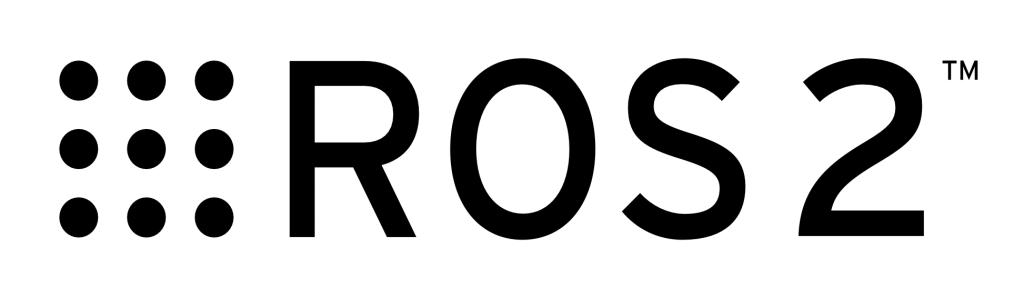
\includegraphics[width=0.6\textwidth]{Images/Methodologies/ros2_logo.png}
    \caption{Robot Operating System 2}
\end{figure}

ROS 2 là một trong những hệ thống hỗ trợ điều khiển robot không thể thiếu trong mọi ứng dụng thiết kế, phát triển và lập trình robot. Việc xây dựng ứng dụng điều khiển cánh tay sử dụng ROS là mục tiêu mà đề tài hướng tới trong giai đoạn tiếp theo. Ở giai đoạn hiện tại, do giới hạn về thời gian dùng để lắp ráp robot, chương trình điều khiển được xây dựng bằng Python ở mức cơ bản để chứng minh khả năng điều khiển và quan sát cách hoạt động thực tế của robot.

\subsection{Ros2-Control}

Ros2-Control là một framework cho việc điều khiển robot thời gian thực (real-time) trên nền tảng ROS2. Mục tiêu chính của Ros2-Control đó là thực hiện việc quản lý và điều khiển phần cứng của robot theo cách thức chuẩn hóa và mô dun hóa, qua đó giúp dễ dàng tích hợp phần cứng vào ứng dụng ROS2. Để làm được điều này, Ros2-Control định nghĩa một kiến trúc bao gồm bốn lớp: Controller, Controller Manager, Resource Manager và Hardware component. Sơ đồ kiến trúc theo Ros2-Control được thể hiện bên dưới:

\begin{figure}[H]
    \centering
    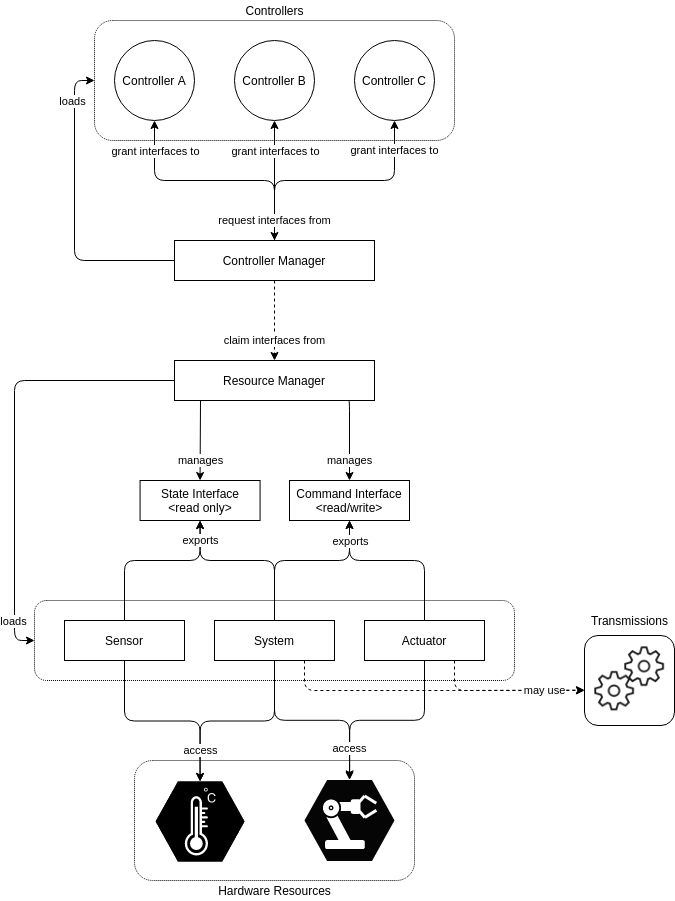
\includegraphics[width=0.9\textwidth]{Images/Methodologies/ros2_control_architect.png}
    \caption{Sơ đồ kiến trúc của Ros2-Control}
\end{figure}

\subsubsection{Controller Manager}
Controller Manager là thành phần kết nối các bộ điều khiển với lớp trừu tượng phần cứng trong framework \texttt{ros2\_control}, đồng thời đóng vai trò là điểm truy cập cho người dùng thông qua các dịch vụ ROS. Controller Manager được triển khai dưới dạng một node không có executor để có thể tích hợp vào thiết lập tùy chỉnh, nhưng thường khuyến nghị sử dụng node mặc định trong file \texttt{ros2\_control\_node} thuộc gói \texttt{controller\_manager}. Trong quá trình hoạt động, Controller Manager quản lý việc nạp, kích hoạt, hủy kích hoạt và gỡ bỏ các bộ điều khiển cùng với các \textbf{interface} mà chúng yêu cầu, đồng thời truy cập vào các thành phần phần cứng thông qua Resource Manager. Controller Manager đối chiếu giữa \textbf{interface} yêu cầu và \textbf{interface} cung cấp, cho phép bộ điều khiển truy cập phần cứng khi được bật hoặc báo lỗi nếu có xung đột. Vòng lặp điều khiển được thực thi bởi phương thức \texttt{update()}, nơi Controller Manager đọc dữ liệu từ phần cứng, cập nhật đầu ra của các bộ điều khiển đang hoạt động và ghi kết quả trở lại phần cứng.

\subsubsection{Resource Manager}
Resource Manager đảm nhận việc trừu tượng hóa phần cứng vật lý và driver của nó, gọi là \textit{hardware components}, cho framework \texttt{ros2\_control}. Resource Manager nạp các thành phần bằng thư viện \texttt{pluginlib}, quản lý vòng đời, trạng thái và \textbf{interface} lệnh của chúng. Nhờ lớp trừu tượng này, các thành phần phần cứng đã triển khai có thể được tái sử dụng mà không cần viết lại, đồng thời cho phép ứng dụng phần cứng linh hoạt cho \textbf{interface} trạng thái và lệnh. Trong vòng lặp điều khiển, Resource Manager giao tiếp với phần cứng thông qua các phương thức \texttt{read()} và \texttt{write()}.

\subsubsection{Controllers}
Các bộ điều khiển trong \texttt{ros2\_control} dựa trên lý thuyết điều khiển, so sánh giá trị tham chiếu với đầu ra đo được và tính toán đầu vào hệ thống dựa trên sai số. Chúng là các đối tượng kế thừa từ \texttt{ControllerInterface} trong gói \texttt{controller\_interface} và được xuất dưới dạng plugin bằng \texttt{pluginlib}. Ví dụ điển hình là \texttt{ForwardCommandController} trong repository \texttt{ros2\_controllers}. Vòng đời của bộ điều khiển dựa trên lớp \texttt{LifecycleNode}, vốn triển khai máy trạng thái được mô tả trong tài liệu \textit{Node Lifecycle Design}. Khi vòng lặp điều khiển chạy, phương thức \texttt{update()} được gọi để truy cập trạng thái phần cứng mới nhất và cho phép bộ điều khiển ghi dữ liệu vào \textbf{interface} lệnh phần cứng.

\subsubsection{Hardware Components}
Các thành phần phần cứng thực hiện giao tiếp với phần cứng vật lý và đại diện cho lớp trừu tượng của nó trong framework \texttt{ros2\_control}. 
Các thành phần này phải được xuất dưới dạng plugin bằng \texttt{pluginlib}. 
Resource Manager sẽ nạp động các plugin này và quản lý vòng đời của chúng.

Có ba loại thành phần cơ bản cho Hardware component:

\begin{itemize}
\item \textbf{{Hệ thống - System}}

Dùng cho phần cứng robot phức tạp (multi-DOF) như robot công nghiệp. Khác với Actuator, System có thể sử dụng truyền động phức tạp như là cánh tay robot hay bàn tay robot (humanoid robot's hand). Hardware component dạng System có khả năng đọc và ghi xuống thiết bị thực tế, và thường dùng khi chỉ có một kênh giao tiếp logic với phần cứng.

\item \textbf{{Cảm biến - Sensor}}
Dành cho phần cứng robot dùng để cảm nhận môi trường xung quanh như camera, cảm biến nhiệt độ, cảm biến màu sắc, không gian.... Các cảm biến thường chỉ Liên kết với một khớp. Đối với hardware dạng cảm biến, ta chỉ có thể đọc dữ liệu được truyền lên từ phần cứng

\item \textbf{{Bộ truyền động - Actuator}}
Bộ truyền động thường nói đến phần cứng robot đơn giản (1 trục tự do) như động cơ, van, v.v.  và chỉ liên kết với một khớp duy nhất. 
tương tự như System, Actuator cũng có khả năng đọc và ghi, tuy nhiên thao tác(\textit{đọc} không bắt buộc nếu không khả thi, ví dụ: điều khiển động cơ DC hay servo 
\end{itemize}

\subsection{MoveIt 2}

MoveIt 2 là một nền tảng phát triển tích hợp trong ROS 2, bao gồm nhiều gói chức năng phục vụ cho việc điều khiển cánh tay robot. Các chức năng này trải rộng từ lập kế hoạch chuyển động, thao tác, điều khiển, động học ngược, nhận thức 3D cho đến phát hiện va chạm, là một nền tảng trợ giúp đắc lực cho việc nhanh chóng xây dựng ứng dụng điều khiển cánh tay robot.

\begin{figure}[H]
    \centering
    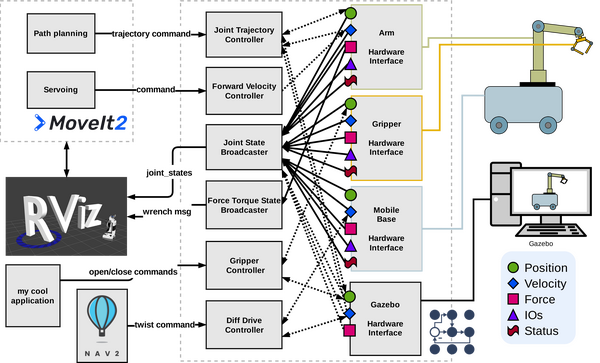
\includegraphics[width=1\textwidth]{Images/Methodologies/moveit_integration.png}
    \caption{MoveIt 2 được tích hợp cùng với Ros2-Control trong ứng dụng robotic}
\end{figure}

MoveIt 2 cung cấp khả năng lập kế hoạch chuyển động dựa trên OMPL (Open Motion Planning Library) cùng nhiều thư viện bên thứ ba, hỗ trợ đa dạng thuật toán và ràng buộc.  
Hệ thống động học ngược (IK) được triển khai thông qua cơ chế plug-in, cho phép sử dụng nhiều bộ giải IK khác nhau để nhanh chóng tính toán tư thế mục tiêu của cánh tay robot.  
Khả năng phát hiện và tránh va chạm được tích hợp sẵn, đảm bảo robot không va chạm với môi trường xung quanh trong quá trình lập kế hoạch và thực thi chuyển động.  
MoveIt 2 còn hỗ trợ cập nhật mô hình môi trường một cách linh hoạt, có thể nhận biết sự thay đổi của chướng ngại vật theo thời gian thực.  
Giao diện điều khiển chuyển động được kết nối chặt chẽ với phần cứng robot, giúp đảm bảo đường đi đã được lập kế hoạch có thể thực hiện chính xác.  
Ngoài ra, MoveIt 2 tích hợp với RViz 2, mang lại công cụ trực quan để tương tác, gỡ lỗi và hiển thị quá trình lập kế hoạch cũng như thực thi chuyển động ngay lập tức.

MoveIt 2 mang lại nhiều ưu điểm trong ứng dụng điều khiển robot với ROS2 như:
\begin{itemize}
    \item Nhờ kiến trúc truyền thông DDS của ROS 2, MoveIt 2 đạt được hiệu năng thời gian thực và độ tin cậy cao hơn đáng kể. 
    \item Thiết kế theo mô-đun giúp người dùng dễ dàng tải hoặc thay thế các thành phần khi cần, mang lại sự linh hoạt lớn.  
    \item MoveIt 2 có khả năng chạy trên nhiều hệ điều hành khác nhau như Ubuntu, Windows, cũng như nhiều nền tảng phần cứng.
    \item Cộng đồng phát triển toàn cầu của MoveIt 2 luôn tích cực đóng góp, liên tục cập nhật, mở rộng tính năng và cung cấp hỗ trợ kỹ thuật.
\end{itemize}

\section{Kính thực tế ảo Meta Quest 3}

\begin{figure}[H]
    \centering
    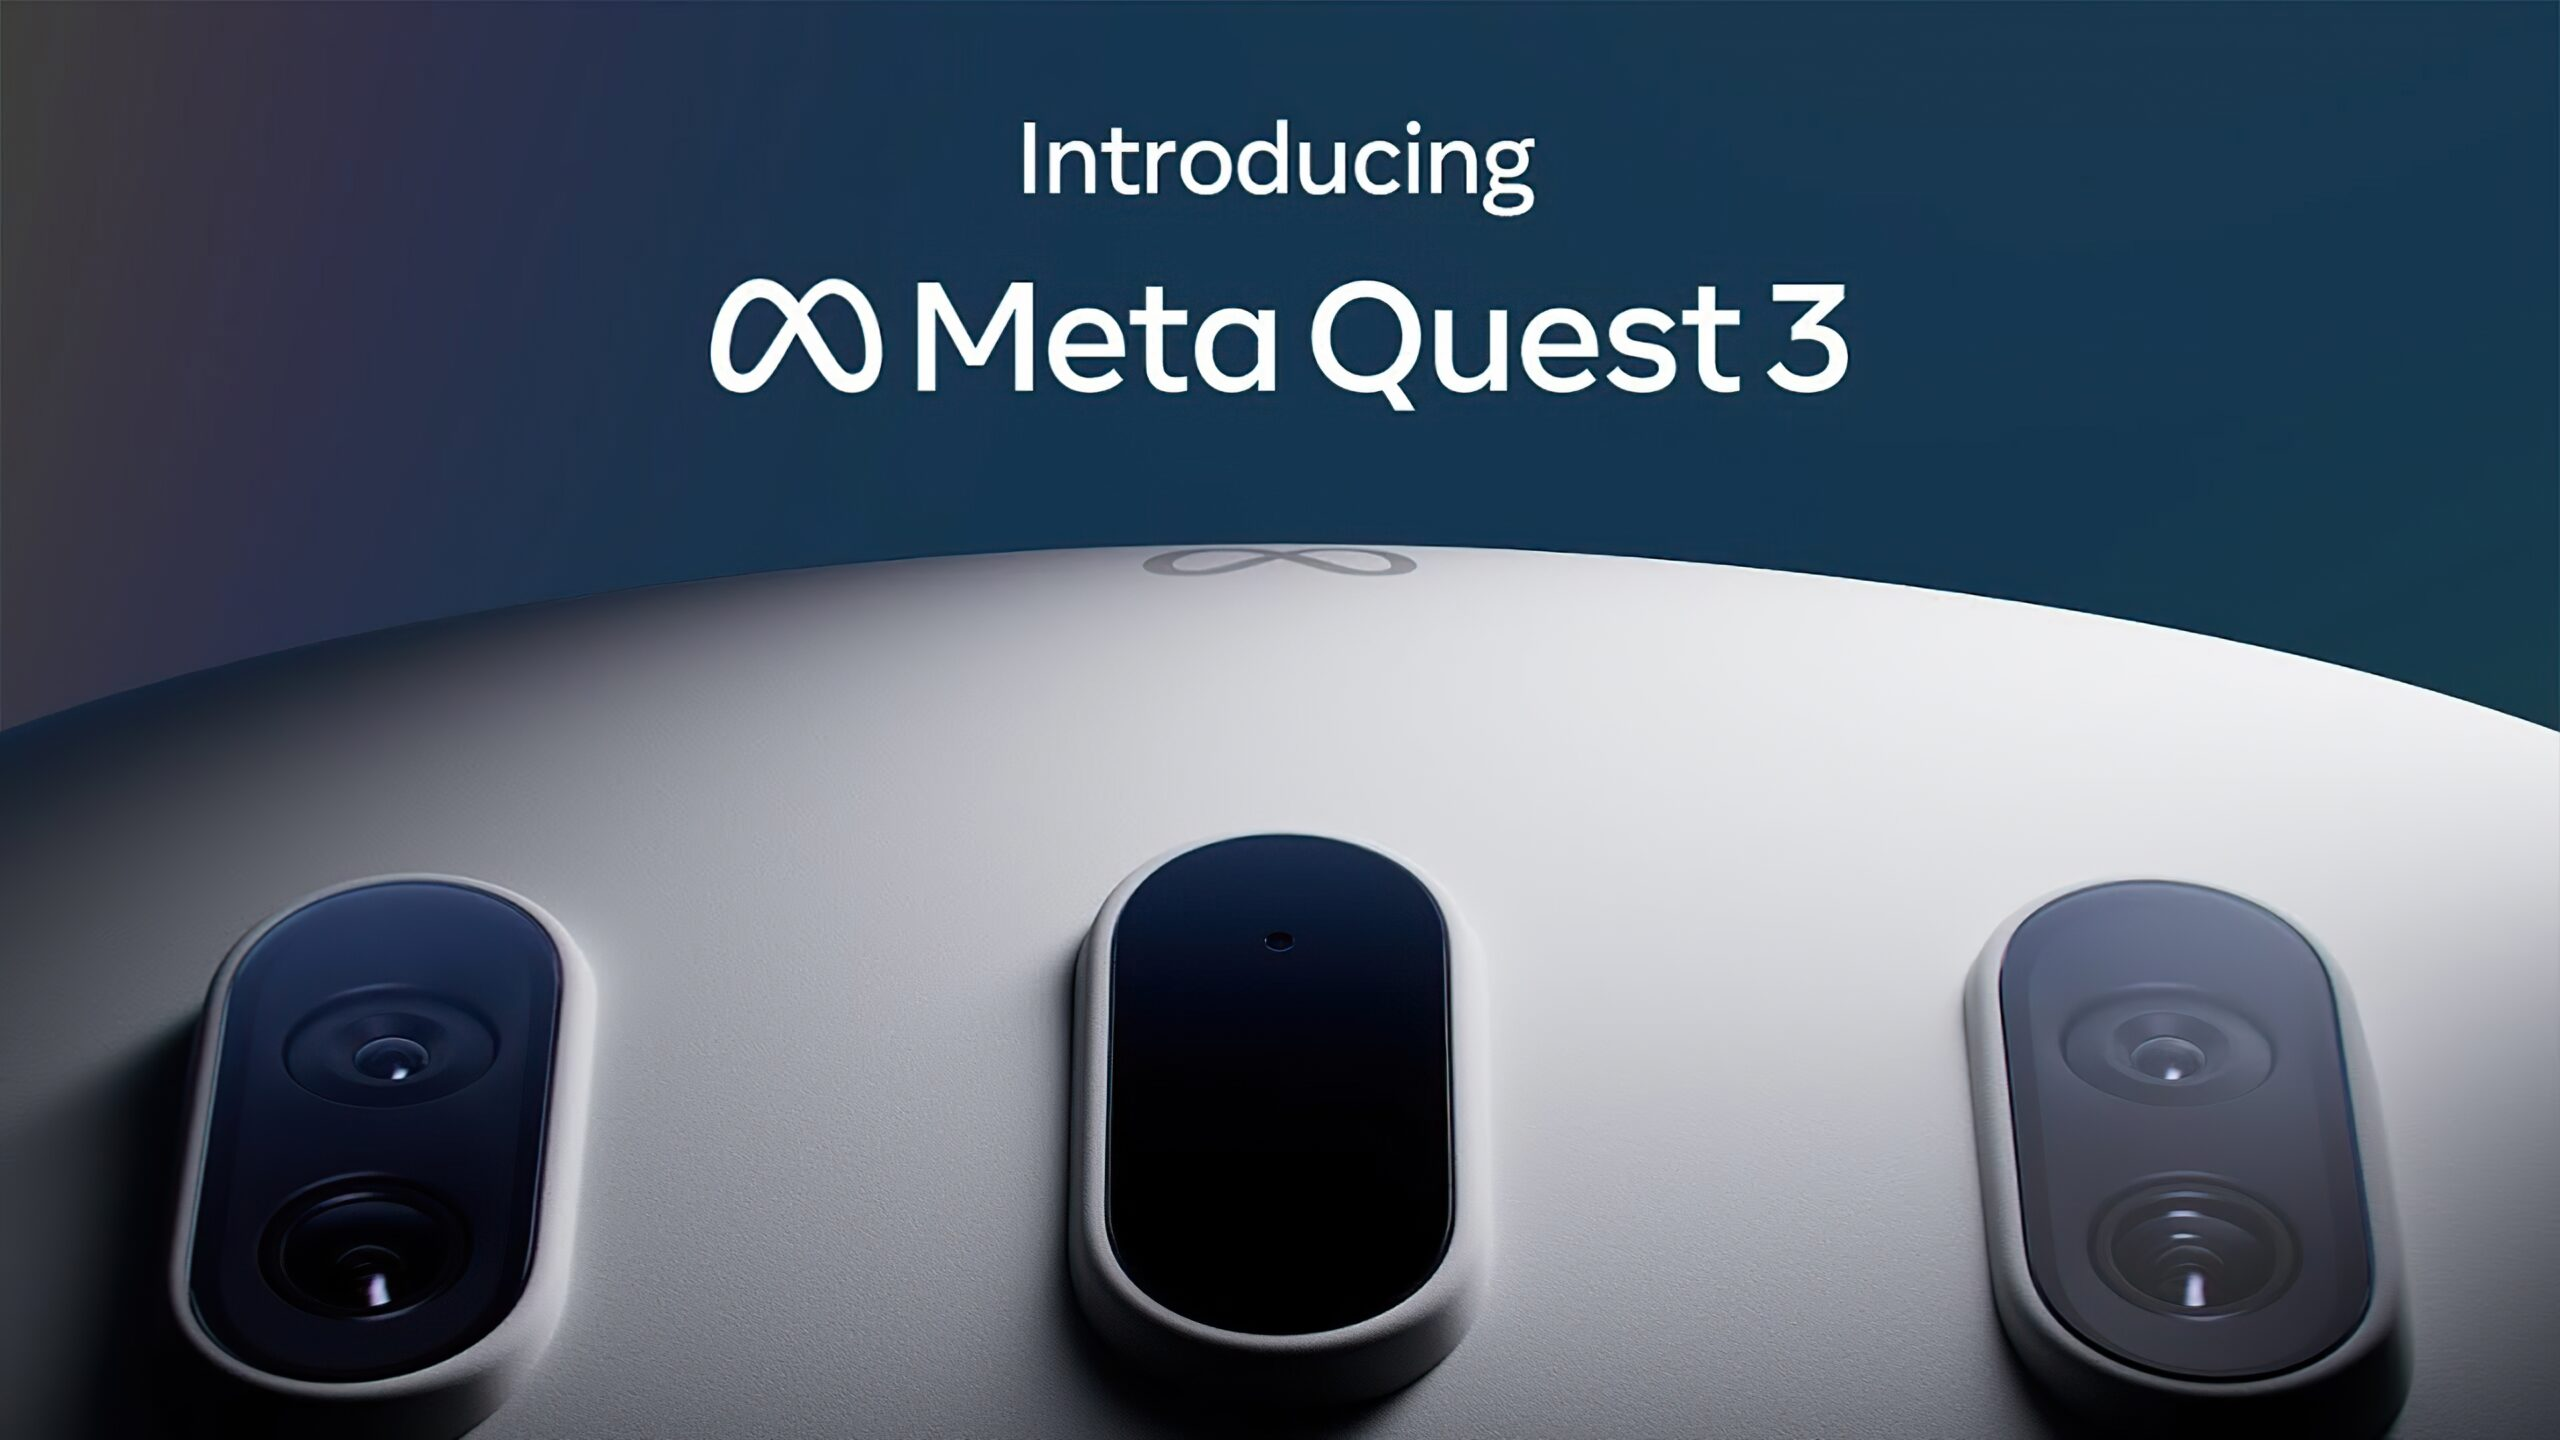
\includegraphics[width=1\textwidth]{Images/Methodologies/meta_quest_3.jpg}
    \caption{Kính thực tế ảo Meta Quest 3}
\end{figure}

Meta Quest 3 là một kính thực tế ảo/ thực tế tăng cường độc lập (standalone VR/MR), là phiên bản mới nhất trong chuỗi thiết bị thực tế ảo được sản xuất bởi Meta. Meta Quest 3 được thiết kế như một thiết bị thực tế ảo nhỏ gọn nhưng mạnh mẽ, cung cấp trải nghiệm tuyệt vời cho người sử dụng thông thường với mức giá hợp lý. Về hiệu năng, Meta Quest 3 trang bị cho mình chip Snapdragon XR2 Gen 2, đem lại gấp đôi hiệu năng xử lý đồ họa, giúp tăng đáng kể thời gian tải ứng dụng và đem lại trải nghiệm mượt mà hơn nhiều so với phiên bản tiền nhiệm Oculus Quest 2. 

Về dung lượng bộ nhớ, Meta Quest 3 sở hữu bộ nhớ mặc định là 512GB, cho phép người dùng có thể thoải mái lưu trữ các tài nguyên, phần mềm và video ưa thích. Ngoài ra, điểm nổi bật của phiển bản Quest 3 hiện tại là khả năng nhìn xuyên kính (passthrough). Với vai trò là một kính thực tế ảo (VR) kiêm thực tế tăng cường (XR), Quest 3 cho phép người dùng đang đeo kính có thể thấy được không gian bên ngoài rõ ràng, một cải tiến tuyệt vời so với phiên bản Oculus 2. 

Ngoài ra, với âm thanh 3D tích hợp trong kính cùng với lượng RAM 8GB, đem lại hiệu năng cao và phù hợp để trải nghiệm mọi ứng dụng ưa thích.

\section{Unity Engine}

Unity là một \textbf{game engine} và nền tảng phát triển ứng dụng đa nền tảng được phát triển bởi Unity Technologies, ra đời từ năm 2005 và hiện là một trong những engine được sử dụng rộng rãi nhất thế giới không chỉ trong lĩnh vực game mà còn trong mô phỏng, đào tạo, kiến trúc, y tế và robot học. Unity hỗ trợ xuất bản ứng dụng trên hơn 20 nền tảng khác nhau, bao gồm PC, Android, iOS, WebGL, và đặc biệt là các thiết bị thực tế ảo (VR) như Meta Quest, HTC Vive, PlayStation VR.

\begin{figure}[H]
    \centering
    
\includegraphics[width=0.8\textwidth]{Images/Methodologies/unity_logo.jpg}
    \caption{Unity Engine}
    \label{fig:unity_logo}
\end{figure}

\textbf{Kiến trúc cơ bản của Unity}

Unity sử dụng mô hình lập trình hướng thành phần (Component-Based Architecture), trong đó mọi đối tượng trong cảnh (scene) đều là một \lstinline[style=inlinecode]{GameObject}. Tính năng và hành vi của đối tượng được xác định bởi các \lstinline[style=inlinecode]{Component} gắn vào nó - ví dụ: \lstinline[style=inlinecode]{Transform} (vị trí, góc xoay, tỷ lệ), \lstinline[style=inlinecode]{Renderer} (hiển thị hình ảnh), \lstinline[style=inlinecode]{Collider} (va chạm vật lý), hay các script C\# tùy biến. Ngôn ngữ lập trình chính thức duy nhất của Unity là \textbf{C\#}, cho phép lập trình viên viết logic, xử lý sự kiện và tương tác với toàn bộ API của engine.

\textbf{Hỗ trợ phát triển VR/MR với Meta SDK}

Để phát triển ứng dụng thực tế ảo cho thiết bị Meta Quest 3, Unity tích hợp trực tiếp với \textbf{Meta XR SDK} (trước đây là Oculus Integration). SDK này cung cấp:

\begin{itemize}
    \item Các \lstinline[style=inlinecode]{Prefab} và component sẵn có cho camera VR, tay cầm (controllers) và tính năng passthrough (xem xuyên kính).
    \item Hệ thống \textbf{XR Interaction Toolkit} hỗ trợ các tương tác tay cầm như grab (cầm nắm), poke (chạm), teleport (dịch chuyển).
    \item Tích hợp với hệ thống \textbf{OVRInput} để đọc trạng thái các nút bấm, joystick và cảm biến tay cầm một cách đơn giản.
    \item Hỗ trợ \textbf{hand tracking} nhận dạng và theo dõi cử chỉ bàn tay người dùng mà không cần tay cầm.
\end{itemize}

\textbf{Vai trò của Unity trong đề tài}

Trong đề tài này, Unity Engine được sử dụng để xây dựng \textbf{ứng dụng VR điều khiển cánh tay robot từ xa}. Ứng dụng kết nối với hệ thống ROS2 thông qua thư viện ROS-Sharp và giao thức WebSocket của RosBridge, cho phép người dùng đeo kính Meta Quest 3 để:

\begin{itemize}
    \item Theo dõi trạng thái cánh tay robot thực tế theo thời gian thực thông qua mô hình 3D đồng bộ.
    \item Xem hình ảnh camera từ môi trường làm việc của robot.
    \item Điều khiển cánh tay bằng tay cầm VR với chế độ real-time servoing.
    \item Lập kế hoạch và thực thi quỹ đạo di chuyển qua giao diện tương tác trực quan.
    \item Điều khiển đóng/mở tay gắp.
\end{itemize}

\section{ROS-Sharp (ROS\#)}

ROS-Sharp (hay ROS\#) là một thư viện mã nguồn mở được phát triển bởi Siemens AG, cung cấp khả năng \textbf{giao tiếp hai chiều giữa Unity và hệ thống ROS/ROS2} thông qua giao thức \textbf{WebSocket} và chuẩn \textbf{ROSBridge Protocol}. Thư viện này cho phép các ứng dụng Unity subscribe và publish các ROS topic, gọi các ROS service và gửi/nhận Action goals mà hoàn toàn không cần cài đặt ROS trực tiếp trên máy chạy Unity.

\begin{figure}[H]
    \centering
    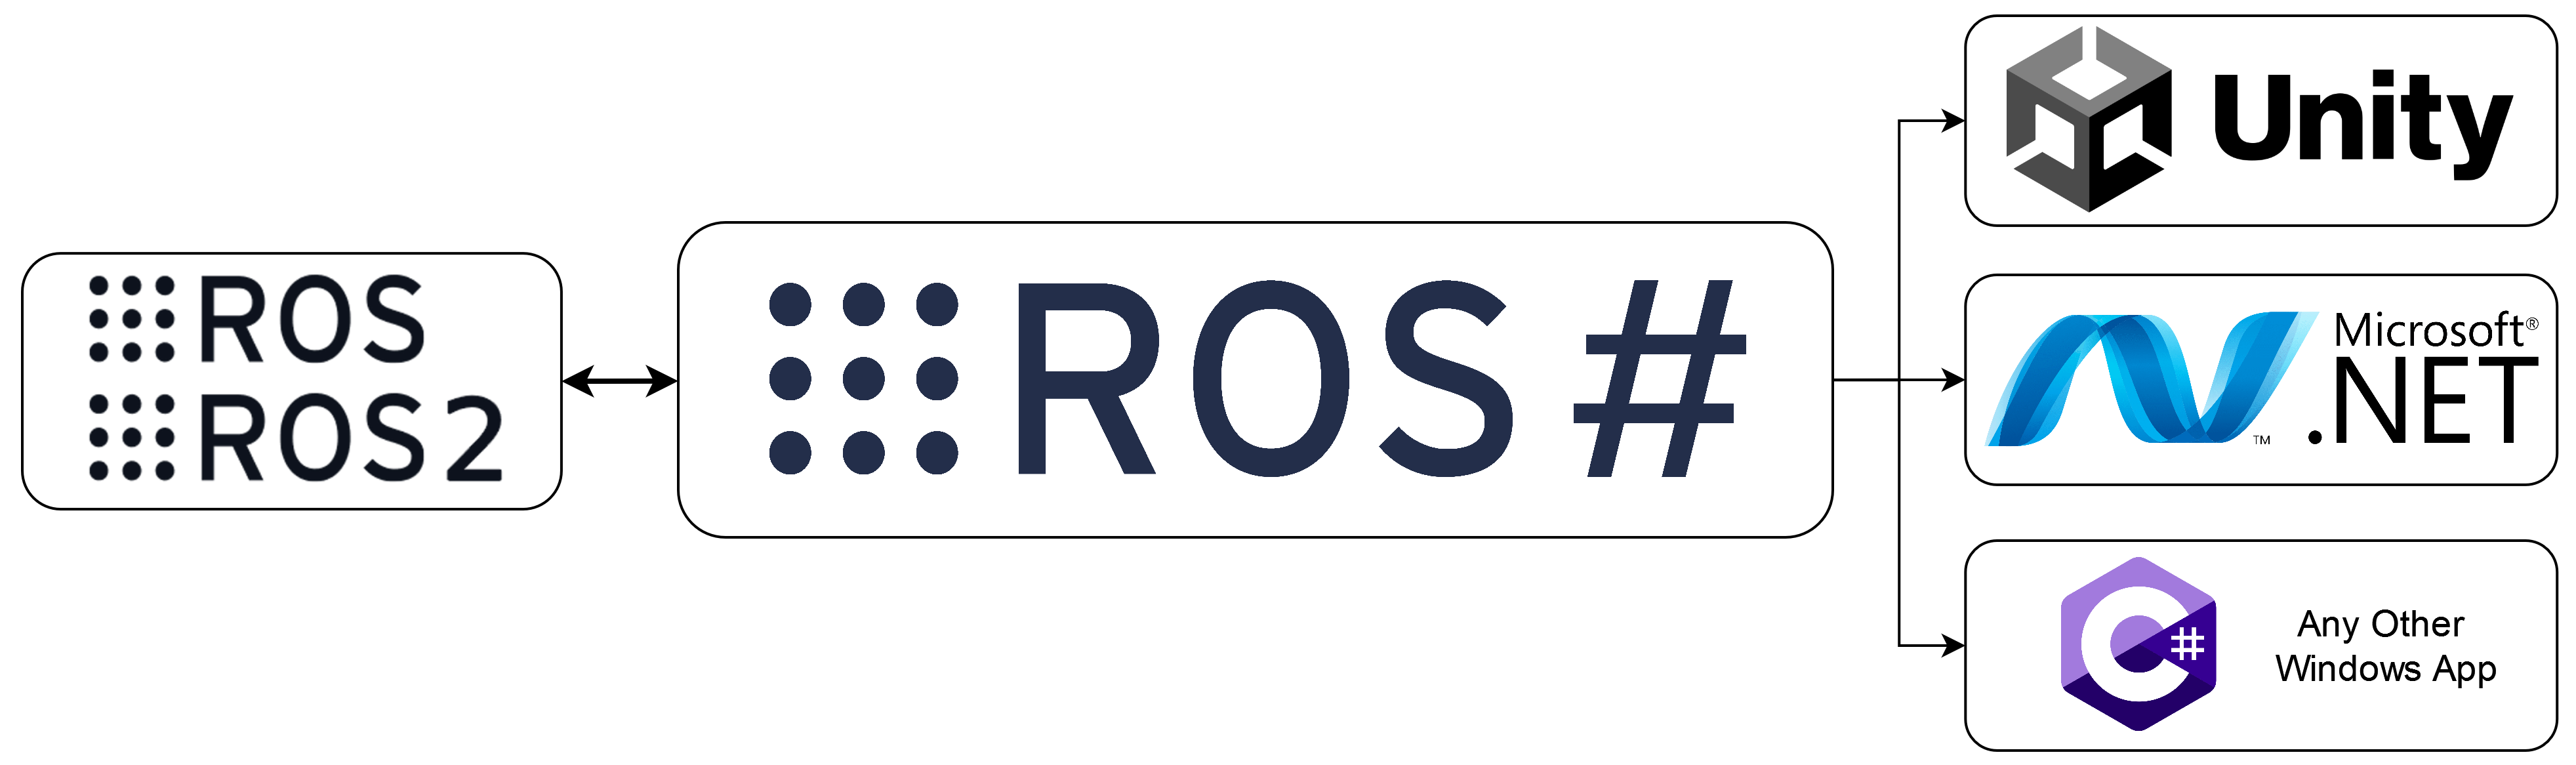
\includegraphics[width=0.8\textwidth]{Images/Methodologies/rossharp_architecture.png}
    \caption{Kiến trúc giao tiếp của ROS-Sharp giữa Unity và ROS2}
    \label{fig:rossharp}
\end{figure}

\textbf{Kiến trúc hoạt động}

ROS-Sharp hoạt động theo mô hình client-server:

\begin{itemize}
    \item \textbf{Phía ROS2 (Server)}: \lstinline[style=inlinecode]{rosbridge_server} lắng nghe kết nối WebSocket tại cổng mạng được cấu hình (mặc định 9090). Mọi thông điệp ROS2 (topic, service, action) đều được serialize sang định dạng JSON theo chuẩn \textit{rosbridge protocol v2.0}.
    \item \textbf{Phía Unity (Client)}: ROS-Sharp cung cấp class \lstinline[style=inlinecode]{RosConnector} thiết lập kết nối WebSocket tới rosbridge server. Từ đó, các script C\# có thể sử dụng các class \lstinline[style=inlinecode]{Subscriber<T>}, \lstinline[style=inlinecode]{Publisher<T>}, \lstinline[style=inlinecode]{ServiceProvider<TReq, TResp>} để tương tác với bất kỳ kênh giao tiếp ROS2 nào.
\end{itemize}

\textbf{Các tính năng chính của ROS-Sharp}

\begin{itemize}
    \item \textbf{Topic Communication}: Publish và subscribe các ROS2 topic với kiểu dữ liệu tương ứng (ví dụ: \lstinline[style=inlinecode]{JointState}, \lstinline[style=inlinecode]{TwistStamped}, \lstinline[style=inlinecode]{Image}). ROS-Sharp tự động serialize/deserialize JSON thành các đối tượng C\# tương ứng.
    \item \textbf{Service Call}: Gọi các ROS2 service từ Unity và nhận kết quả phản hồi không đồng bộ.
    \item \textbf{Action Goal}: Gửi Action goal và nhận Feedback, Result của ROS2 Action thông qua WebSocket.
    \item \textbf{URDF Importer}: Một tính năng quan trọng của ROS-Sharp là khả năng \textbf{import mô hình robot từ URDF} trực tiếp vào Unity. Kết hợp với \lstinline[style=inlinecode]{file_server} package phía ROS2, Unity có thể tải toàn bộ file URDF cùng các file mesh (\lstinline[style=inlinecode]{.dae}, \lstinline[style=inlinecode]{.stl}) về và dựng lại mô hình 3D đầy đủ của robot trong scene VR.
\end{itemize}

\textbf{Vai trò trong đề tài}

Trong đề tài, ROS-Sharp là cầu nối thiết yếu giúp ứng dụng Unity VR kết nối với toàn bộ stack điều khiển ROS2 đã xây dựng. Cụ thể, các kênh giao tiếp được sử dụng bao gồm:

\begin{itemize}
    \item Subscribe topic \lstinline[style=inlinecode]{/joint_states} để cập nhật liên tục trạng thái góc xoay của cánh tay, đồng bộ mô hình 3D trong VR với robot thực tế.
    \item Subscribe topic \lstinline[style=inlinecode]{/image_raw} (hoặc topic camera tương ứng) để hiển thị luồng video từ camera gắn trên robot.
    \item Gửi Action goal tới \lstinline[style=inlinecode]{move_to_pose} (module Denso Remote Control) để lập kế hoạch và thực thi quỹ đạo di chuyển.
    \item Gọi service \lstinline[style=inlinecode]{~/start_servo} / \lstinline[style=inlinecode]{~/stop_servo} để bật/tắt chế độ MoveIt Servo.
    \item Publish topic \lstinline[style=inlinecode]{~/delta_joint_cmds} hoặc \lstinline[style=inlinecode]{~/delta_twist_cmds} để gửi lệnh điều khiển real-time trong chế độ Servo.
    \item Gửi Action goal tới \lstinline[style=inlinecode]{gripper_cmd} (denso\_hand\_controller) để điều khiển đóng/mở tay gắp.
\end{itemize}

Nhờ ROS-Sharp và rosbridge\_server, toàn bộ logic điều khiển phức tạp nằm ở phía ROS2, còn Unity chỉ cần đảm nhiệm phần giao diện người dùng và trải nghiệm VR, tạo ra sự phân tách rõ ràng và linh hoạt trong kiến trúc hệ thống.